% !TeX spellcheck = en_GB
\begin{figure}
  \setlength{\unitlength}{\textwidth}

        \begin{picture}(1,0.48)(-0.02,0)


      
      \put(0.08,0.08){\includegraphics[width=0.75\unitlength]{./chapter-pi_1_pi_2/FnP/gnuplot/displacement_amp_re200_col.eps}}


      \put(0.46,0.04){$\displaystyle\frac{2\sqrt{\massstiff}}{\massdamp\mstar }\ustar$}
      
      
     
       \put(0.022,0.28){$\displaystyle\frac{2\sqrt{\massstiff}}{\massdamp\mstar } \frac{A}{D}$}
      

      %\put(0.095,0.218){\small(a)}
      %\put(0.565,0.218){\small(b)}
      
    \end{picture}

  \caption{Displacement amplitude data as function of $\ustar$. obtained at $Re=200$ and $m^*=20$ at three different damping ratios: $\zeta=0.075$ ($\times$), $\zeta=0.1$ (\ding{117}) and $\zeta=0.15$ (+). Both the independent and dependent variables are scaled with $\frac{2\sqrt{\massstiff}}{\massdamp\mstar }$  which is equal to $\frac{1}{\mstar\zeta}$. This scaling is similar to \cite{Parkinson1964} and the deviation of data using this scaling at high \ustar could be observed in  \cite{Parkinson1964}}
    \label{fig:amp-collapsed}
\end{figure}

 %vspace{10cm}
